\section{Errors with the Parallel Merge}
It was noted that merges generated on the GPU differed slightly from those generated using the sequential algorithm. While the error increases for both are almost equal, the slight variances lead to different final tessellations for the same set of sources. This can be seen in the differences between Figure \ref{gpu:fig:seqm} generated using the sequential merge and Figure \ref{gpu:fig:parm} generated from the GPU algorithm. The reason for this is most likely due to the way in which CUDA executes floating point operations on the GPU \citep{CUDA}. While the differences in these calculations lead to slightly varying results, the fact that the global error and number of cells are almost equivalent means that results generated by the GPU are still valid.
\begin{figure}[H]
\centering
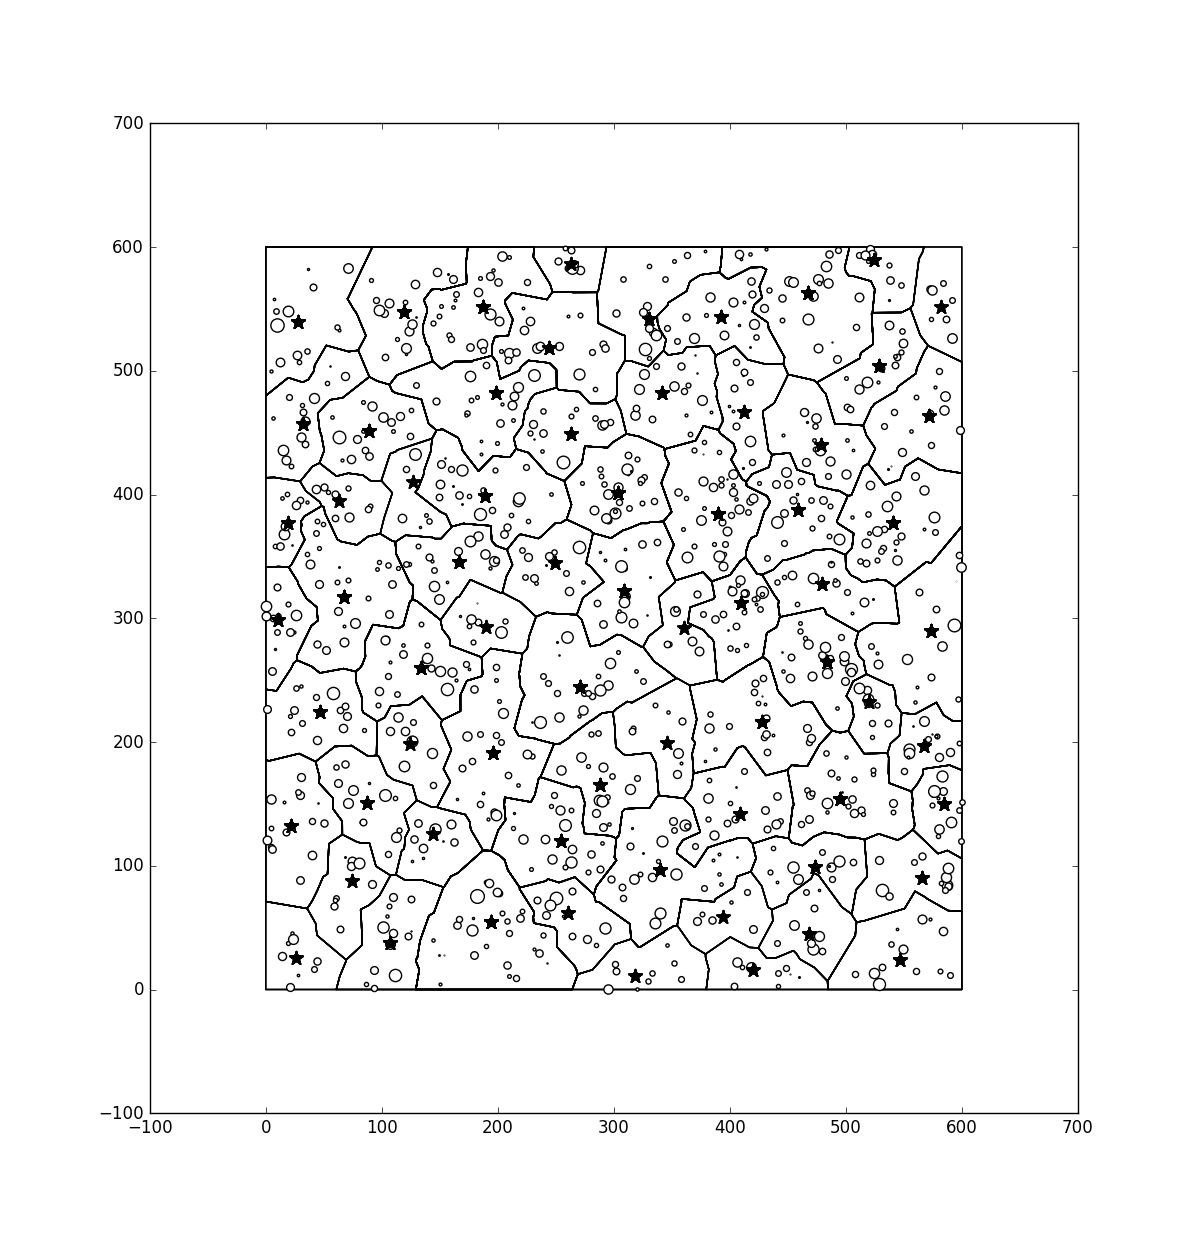
\includegraphics[width=0.6\textwidth]{Images/cpu_merge.png}
\caption{A completed merge tessellation generated with the sequential cell merge algorithm.}
\label{gpu:fig:seqm}
\end{figure}
\begin{figure}[H]
\centering
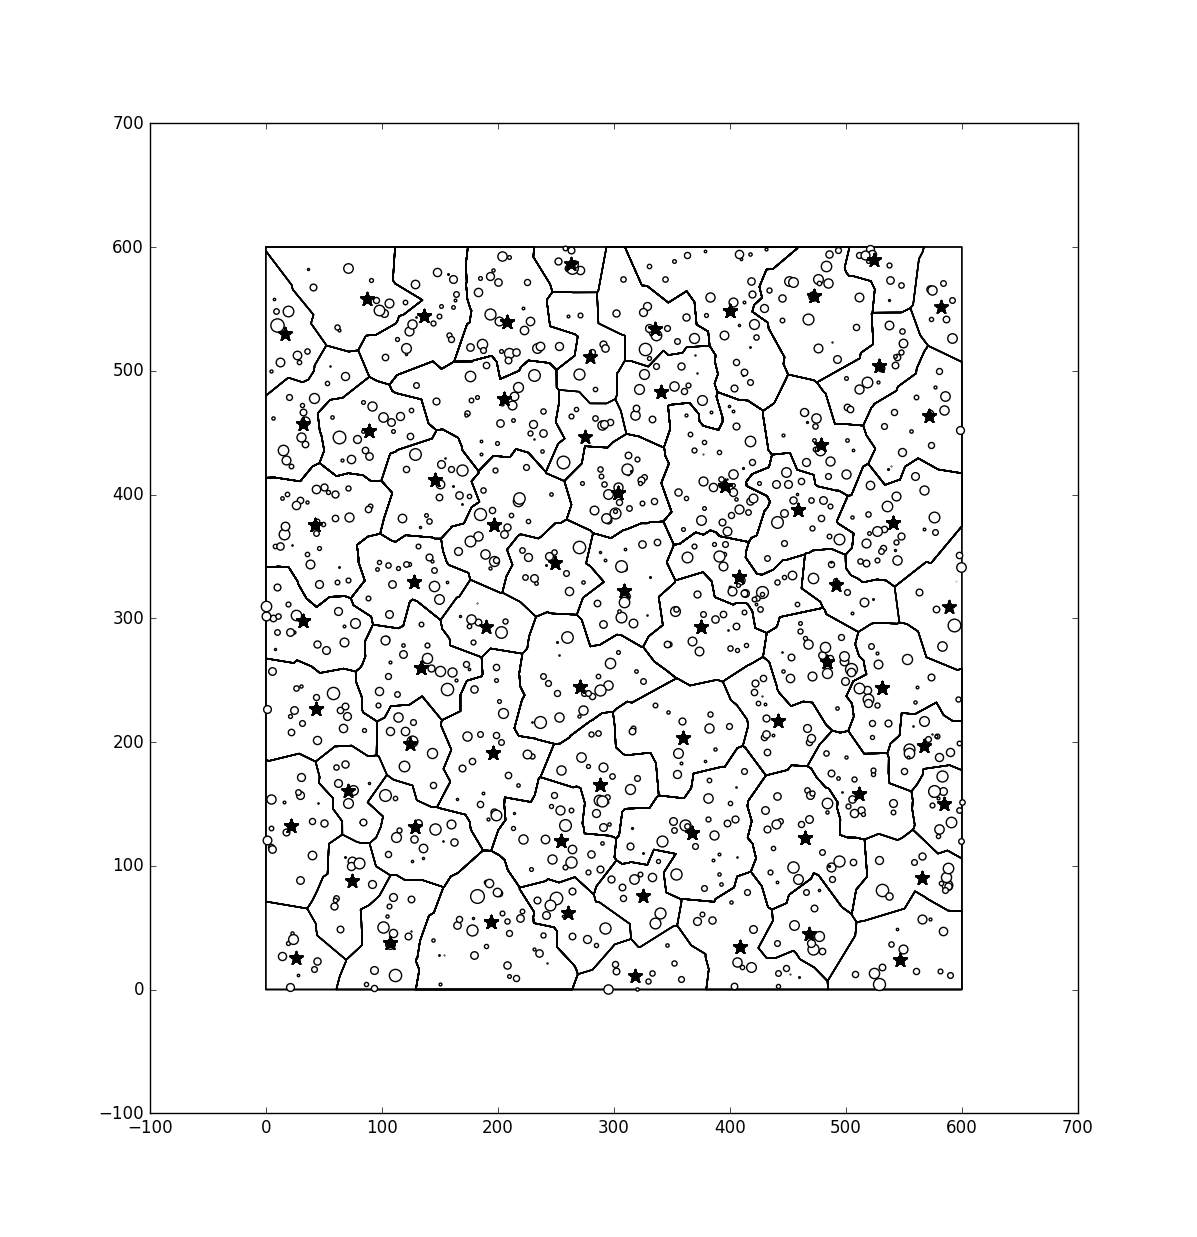
\includegraphics[width=0.6\textwidth]{Images/gpu_merge.png}
\caption{A completed merge tessellation generated with the parallel implementation of the cell merge algorithm.}
\label{gpu:fig:parm}
\end{figure}
